\documentclass[letterpaper,10pt]{article}

\usepackage{geometry}
\usepackage{hyperref}
\usepackage[pdftex]{graphicx}
\usepackage{tikz}
\usepackage{wrapfig}
\geometry{textheight=8.5in, textwidth=6in}
\newenvironment{bottompar}{\par\vspace*{\fill}}{\clearpage}

\title{Requirements For RockSat-X Payload - Hephaestus}
\author{Helena~Bales, Amber~Horvath, and Michael~Humphrey\\ \\ CS461 - Fall 2016}

\parindent = 0.0 in
\parskip = 0.1 in

\begin{document}
\maketitle

\begin{abstract}
The Oregon State University RockSat-X team shall be name Hephaestus.
The requirements for the hardware, software, and programmatic development of Hephaestus shall be outlined in the following document.
The mission requires that the payload, an autonomous robotic arm, perform a series of motions to locate predetermined targets.
The hardware shall be capable of performing the motions to reach the targets.
The software shall determine the targets and send the commands to the hardware to execute the motion.
The combination of the hardware controlled by the software shall demonstrate Hephaestus's ability to construct small parts on orbit.
\end{abstract}

\begin{bottompar}
Approved By
\_\_\_\_\_\_\_\_\_\_\_\_\_\_\_\_\_\_\_\_\_\_\_\_\_\_\_\_\_\_\_\_\_\_\_\_\_\_\_\_\_\_\_\_\_\_\_\_\_\_\_\_\_\_\_\_\_\_\_\_\_\_\_
Date \_\_\_\_\_\_\_\_\_\_\_\_\_\_\_\_\_\_\_\_\_\_\_\_\_\_\_\_ \\


Approved By
\_\_\_\_\_\_\_\_\_\_\_\_\_\_\_\_\_\_\_\_\_\_\_\_\_\_\_\_\_\_\_\_\_\_\_\_\_\_\_\_\_\_\_\_\_\_\_\_\_\_\_\_\_\_\_\_\_\_\_\_\_\_\_
Date \_\_\_\_\_\_\_\_\_\_\_\_\_\_\_\_\_\_\_\_\_\_\_\_\_\_\_\_ \\


Approved By
\_\_\_\_\_\_\_\_\_\_\_\_\_\_\_\_\_\_\_\_\_\_\_\_\_\_\_\_\_\_\_\_\_\_\_\_\_\_\_\_\_\_\_\_\_\_\_\_\_\_\_\_\_\_\_\_\_\_\_\_\_\_\_
Date \_\_\_\_\_\_\_\_\_\_\_\_\_\_\_\_\_\_\_\_\_\_\_\_\_\_\_\_ \\


Approved By
\_\_\_\_\_\_\_\_\_\_\_\_\_\_\_\_\_\_\_\_\_\_\_\_\_\_\_\_\_\_\_\_\_\_\_\_\_\_\_\_\_\_\_\_\_\_\_\_\_\_\_\_\_\_\_\_\_\_\_\_\_\_\_
Date \_\_\_\_\_\_\_\_\_\_\_\_\_\_\_\_\_\_\_\_\_\_\_\_\_\_\_\_ \\
\end{bottompar}

\clearpage
\tableofcontents
\clearpage

\section{Introduction}
\subsection{Purpose of Document}
This document shall describe in detail the Hephaestus RockSat-X payload.
It shall specify the software behavior of the payload.
This document will not discuss the specific implementations of the hardware or the software.
It will specify the behavior by describing the Functional and Non Functional requirements of the software.
This document will be updated throughout the project and should be considered a living document.

\subsection{Overview of Document}
This document will first cover the functional requirements of the project, then the non functional requirements.
The Functional Requirements will include descriptions of the main behavior, target generation, movement, operation modes, and telemetry.
Each of these topics will include descriptions of the behavioral requirements for each.
The Non Functional requirements will cover the performance, security, and telemetry.
Each of the non functional topics covered will include the requirements for the quality of each of the topics.

\subsection{Overview of Payload}
The Hephaestus RockSat-X payload is a deployable rocketry payload that will fly on the 2016 RockSat-X launch.
The payload's main function is to provide a proof of concept for delicate construction in a space environment.
The Hephaestus payload shall perform the following operations:
\begin{itemize}
\item{Remain retracted with power off for duration of launch}
\item{Power on at apogee}
\item{Deploy arm assembly body}
\item{Deploy arm}
\item{Perform 360 degree sweep with video camera}
\item{Generate targets for arm motions}
\item{Perform arm motions}
\item{Record each arm motion with video camera}
\item{Retract arm}
\item{Retract arm assembly body}
\item{Power off}
\end{itemize}

\subsection{Overview of Physical Payload}
While this document focuses on the software of the Hephaestus payload, the project also includes hardware
 and electrical systems. 
Understanding the physical appearance of the payload will help with understanding the software system. 
As such, Figure 1 should serve as a reference for the physical appearance of the payload.
\begin{figure}
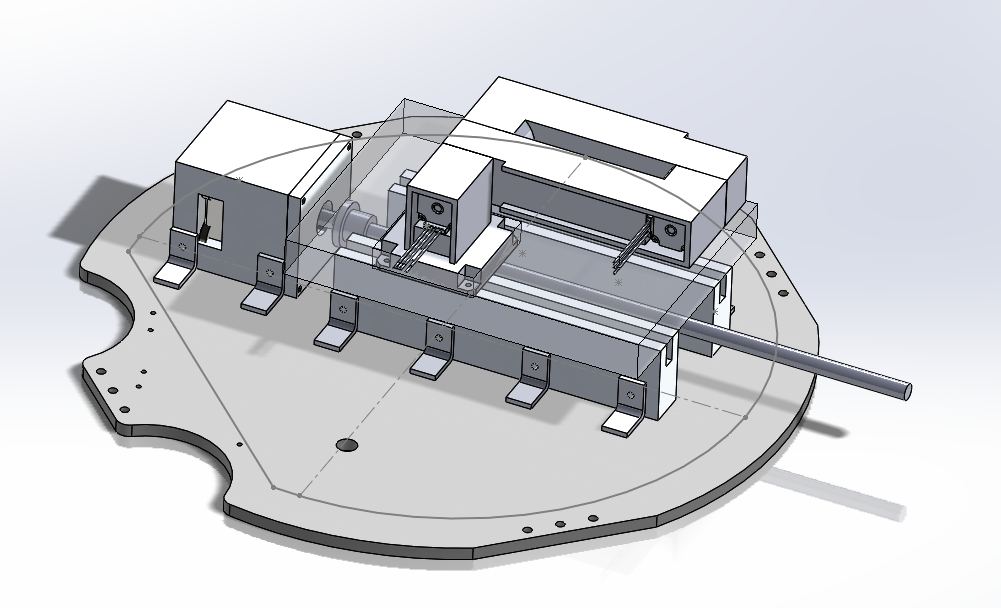
\includegraphics[scale=.5]{img2}
\caption{Model of Hephaestus Payload}
\end{figure}

\subsection{Mission Success Criteria}
The following criteria determine if the Hephaestus mission will be considered successful post-flight.
The minimum mission success criteria represent the lowest criteria to be met in order for the mission to be considered successful.
If the minimum mission success criteria are not met, then the mission may not be considered successful.
The maximum success criteria define the highest goals for the mission.
Fulfilling any or all of these criteria, in addition to the minimum success criteria, would constitute a highly successful mission.
The success of the mission shall be evaluated by means of video recordings recovered post-flight and telemetry data received during the flight.

\subsubsection{Minimum Mission Success Criteria}
\begin{itemize}
\item{The arm assembly body shall deploy and a video sweep is successfully recorded.}
\item{The arm assembly body shall be fully retracted after data collection.}
\end{itemize}

\subsubsection{Maximum Mission Success Criteria}
\begin{itemize}
\item{The arm assembly body shall deploy and a video sweep is successfully recorded.}
\item{The arm shall make contact with predetermined targets around the payload.}
\item{The camera shall record all instances of contact between the arm and the targets.}
\item{The arm assembly body shall be fully retracted after data collection.}
\end{itemize}

\subsection{Requirements Apportioning}

\subsubsection{Priority 1}
This is the highest priority level. In order for the software system to be considered complete and ready for launch, all requirements of this level must be met.
The completion of only Priority 1 requirements marks the completion of Minimum Mission Success criteria, as defined in section 1.4.

\subsubsection{Priority 2}
Requirements of Priority 2 are not required for the release of the software system.
Not completing these requirements must not present a risk to mission success.
The completion of these requirements and successful performance on orbit marks completion of part of the Maximum Success Criteria, as defined in section 1.4.

\subsubsection{Priority 3}
Requirements of Priority 3 are not required for the release of the software system.
Not completing these requirements must not present a risk to mission success.
Completion of all priority 3 requirements and those of higher priority, with successful performance on orbit, marks the completion of the Maximum Mission Success Criteria, as defined in section 1.4.

\section{Functional Requirements}

\subsection{Main Behavior}
\textbf{Priority 1:}
The software shall control the movement of the arm assembly body to make contact with the payload base
at locations generated by the Software (section 2.2). 

\subsection{Target Generation}
\textbf{Priority 1:}
The software shall generate points to be used in testing the Hephaestus arm.
The points will constitute the total test of the arm, and should therefore include points
representative of standard and edge cases.
The points shall be generated in polar form, including an angle from normal, a radius, and a height. 
The angle shall be in the range of 0 and 359 degrees.
An angle of zero degrees shall be in the direction of payload deployment.
The radius shall be the distance from the arm's attachment to the base to the generated point.
The height of the point, for the purpose of target generation, shall be constant.
However the points will always be stored in a triple of angle from normal (\(\theta\)), radius (\(r\)), and height (\(h\)).
These points shall be used as targets for the arm body.

\subsection{Movement}
The software shall control the movement of the arm body assembly. 
The position of the tip of the arm shall be tracked in the coordinate notation described in section 2.2 above.

\textbf{Priority 1:}
The software shall rotate the arm body assembly in a full 360 degrees.

\textbf{Priority 2:}
The software shall additionally control the movement the height of the arm body assembly.
The arm should descend and touch the baseplate of the payload at any rotation.

\subsection{Modes}
During the course of the flight, the software will progress though several different modes of operation.

\subsubsection{Launch}
\textbf{Priority 1:}
The software shall remain idle during launch.

\subsubsection{Deployment}
\textbf{Priority 1:}
The software shall power on the arm assembly body and video camera.
The software shall begin saving the video feed from the camera to a persistent storage location.
The software shall generate target points, as defined in section 2.2.

\subsubsection{Science}
\textbf{Priority 1:}
The software shall collect data to serve as a proof-of-concept for construction of structures in flight.

\subsubsection{Safety}
\textbf{Priority 1:}
The software shall ensure that the arm assembly body can be fully retracted after completing the mission.
The software shall, in case of a failure, eject the arm to prevent damage to the arm assembly body and the rocket during descent.

\subsubsection{Observation}
\textbf{Priority 1:}
The software shall report all telemetry data (as defined in 2.5) to the ground station.

\textbf{Priority 2:}
The software shall be responsible for turning the camera on and off.

\subsubsection{Power Off}
\textbf{Priority 1:}
The software shall power down all subsystems of the payload in preparation for descent.

\subsubsection{State Diagram}
\begin{center}
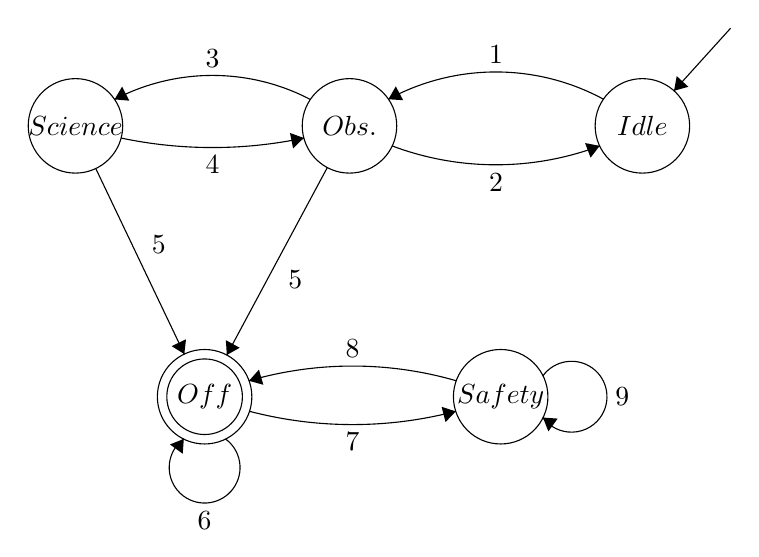
\begin{tikzpicture}[scale=0.2]
\tikzstyle{every node}+=[inner sep=0pt]
\draw [black] (24.2,-19.2) circle (3);
\draw (24.2,-19.2) node {$Obs.$};
\draw [black] (42.8,-19.2) circle (3);
\draw (42.8,-19.2) node {$Idle$};
\draw [black] (6.8,-19.2) circle (3);
\draw (6.8,-19.2) node {$Science$};
\draw [black] (15,-36.4) circle (3);
\draw (15,-36.4) node {$Off$};
\draw [black] (15,-36.4) circle (2.4);
\draw [black] (33.8,-36.4) circle (3);
\draw (33.8,-36.4) node {$Safety$};
\draw [black] (48.4,-13) -- (44.81,-16.97);
\fill [black] (44.81,-16.97) -- (45.72,-16.72) -- (44.98,-16.04);
\draw [black] (26.67,-17.507) arc (118.43354:61.56646:14.344);
\fill [black] (26.67,-17.51) -- (27.61,-17.57) -- (27.14,-16.69);
\draw (33.5,-15.28) node [above] {$1$};
\draw [black] (40.088,-20.475) arc (-69.41442:-110.58558:18.736);
\fill [black] (40.09,-20.47) -- (39.16,-20.29) -- (39.51,-21.22);
\draw (33.5,-22.17) node [below] {$2$};
\draw [black] (9.281,-17.525) arc (117.61533:62.38467:13.416);
\fill [black] (9.28,-17.52) -- (10.22,-17.6) -- (9.76,-16.71);
\draw (15.5,-15.5) node [above] {$3$};
\draw [black] (21.303,-19.973) arc (-78.10445:-101.89555:28.152);
\fill [black] (21.3,-19.97) -- (20.42,-19.65) -- (20.62,-20.63);
\draw (15.5,-21.08) node [below] {$4$};
\draw [black] (8.09,-21.91) -- (13.71,-33.69);
\fill [black] (13.71,-33.69) -- (13.82,-32.75) -- (12.91,-33.19);
\draw (11.61,-26.74) node [right] {$5$};
\draw [black] (16.323,-39.08) arc (54:-234:2.25);
\draw (15,-43.65) node [below] {$6$};
\fill [black] (13.68,-39.08) -- (12.8,-39.43) -- (13.61,-40.02);
\draw [black] (22.79,-21.85) -- (16.41,-33.75);
\fill [black] (16.41,-33.75) -- (17.23,-33.29) -- (16.35,-32.81);
\draw (20.28,-28.97) node [right] {$5$};
\draw [black] (30.948,-37.326) arc (-75.33467:-104.66533:25.865);
\fill [black] (30.95,-37.33) -- (30.05,-37.04) -- (30.3,-38.01);
\draw (24.4,-38.67) node [below] {$7$};
\draw [black] (17.821,-35.385) arc (106.14932:73.85068:23.653);
\fill [black] (17.82,-35.39) -- (18.73,-35.64) -- (18.45,-34.68);
\draw (24.4,-33.95) node [above] {$8$};
\draw [black] (36.48,-35.077) arc (144:-144:2.25);
\draw (41.05,-36.4) node [right] {$9$};
\fill [black] (36.48,-37.72) -- (36.83,-38.6) -- (37.42,-37.79);
\end{tikzpicture}
\end{center}
\begin{center}
State diagram for transition between operational modes.
\end{center}

\subsection{Telemetry}
Let the telemetry interface be defined as 5 of the ten analog pins provided by Wallops Flight Facility.
Let telemetry be defined as the data transmitted from the payload to the ground station via the telemetry interface.
The software shall report all telemetry data to the ground station.

\textbf{Priority 1:}
The software shall report via telemetry all the target points it generates, as defined in section 2.2.
The software shall also report which code branch it takes to facilitate debugging and post-mortem analysis, if necessary. 

\section{Non Functional Requirements}
\subsection{Performance}
\textbf{Priority 1}: The system shall perform efficiently. The maximum response service time should be long enough for the robotic arm to move from one target to another.
 The system should have a maximum throughput that allows for processing of input arguments about the arm's actions and processing for the telemetry data output. 
 Resource usage should be limited to account for the storing of telemetry data. Power consumption must be limited to 28V.
\subsection{Security}
\textbf{Priority 1}: The system shall be secure. Since it is a closed system, the device will be programmed such that it cannot be accessed remotely and will only output sanitized data.
\subsection{Telemetry}
\textbf{Priority 1}: The system will perform telemetry. The data will be transmitted with a delay of up to 10 seconds.

\section{Gantt Chart}
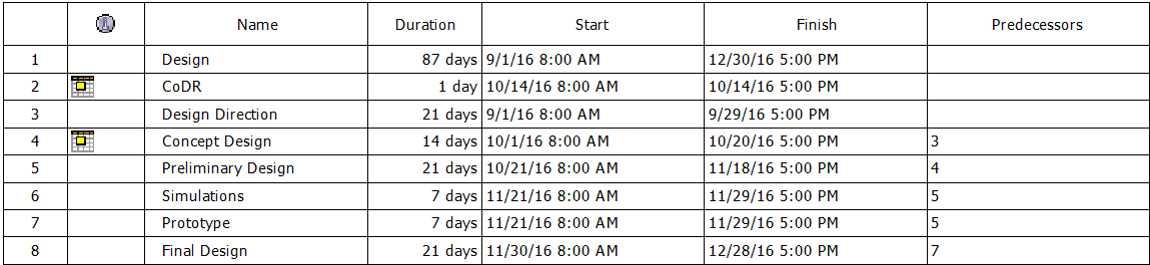
\includegraphics[width=\textwidth]{gantttable}
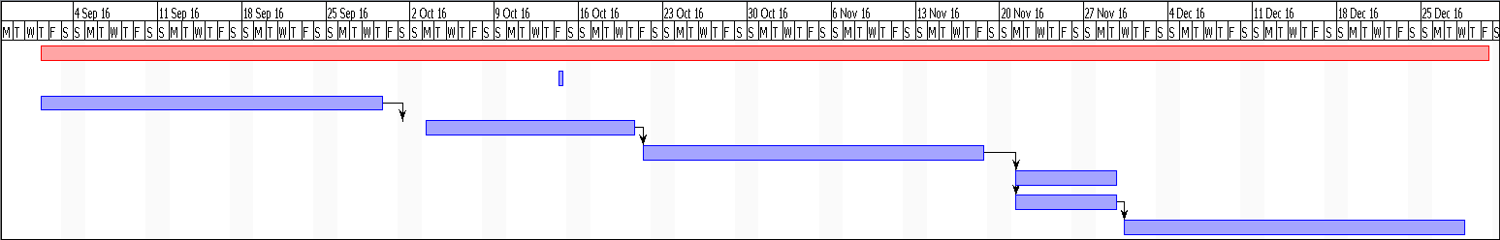
\includegraphics[width=\textwidth]{ganttchart}

\end{document}
